\documentclass[runningheads]{llncs}

\usepackage[T1]{fontenc}
\usepackage[utf8]{inputenc}
\usepackage[numbers,sort&compress]{natbib}
\usepackage{hyperref}
\usepackage{url}
\usepackage{booktabs}
\usepackage{amsfonts}
\usepackage{amsmath}
\usepackage{amssymb}
\usepackage{microtype}
\usepackage{graphicx}
\graphicspath{{../figures/}{./}{../}}
\usepackage{enumitem}

\begin{document}

\title{The Price of Information:\\
$w$ as a Shadow Price on a Sensing Budget}

\titlerunning{The Price of Information}

\author{Patrick Cooper}

\authorrunning{P. Cooper}

\institute{University of Colorado Boulder}

\maketitle

\begin{abstract}
In $\rho$-POMDPs and Expected Free Energy (EFE) planning, information seeking is weighted by a coefficient~$w$. The canonical choice $w{=}1$ is not reward-scale invariant: multiplying all rewards by $\alpha$ leaves the information term unchanged and silently shifts the observe/commit tradeoff. We recast $w$ as an \emph{operational shadow price} of a sensing budget~$B$. Offline, a usage curve $U(w)$ yields a (possibly set-valued) weight $w^*(B)$ that spends about~$B$ observations per episode. Online, a projected dual update adapts~$w$ to hit~$B$, mirroring Soft Actor-Critic's automatic temperature tuning. Three experiments support the account: (i)~usage curves collapse across reward scales when plotted against $w/\alpha$, and crossing brackets in $w/\alpha$ units coincide; (ii)~on deliberately positive-threshold testbeds, the onset of observing matches the closed-form Proposition~2 threshold of the companion IWAI paper to within~$3\%$; (iii)~after a mid-run $\times 10$ reward rescale, dual control re-pins usage and converges into the $\times 10$-scaled offline bracket ($w$ ratio $\approx 9.3$), with lr reset-on-shift cutting re-adaptation from $157$ to $45$ episodes. The construction turns ``choose~$w$'' into ``choose how much sensing to buy.''
\keywords{Active inference \and Expected free energy \and $\rho$-POMDPs \and Sensing budgets \and Shadow prices \and Dual control}
\end{abstract}

%----------------------------------------------------------------------
\section{Introduction}
%----------------------------------------------------------------------

Agents that act under partial observability must decide \emph{how much} information to buy before committing. In $\rho$-POMDPs~\citep{araya2010}, a belief-dependent utility $\rho$ rewards uncertainty reduction alongside task reward; active inference supplies Expected Free Energy (EFE) as a concrete $\rho$ whose information-unit weight is $w{=}1$ under a shared reward convention~\citep{friston2015,parr2019}. That default is empirically near the success--reward knee across a broad observe-then-commit and inspection suite~\citep{cooper2026efe}, but it is \emph{not} scale invariant: if every reward and cost is multiplied by $\alpha>0$, the bit-valued information term is unchanged, so fixed $w{=}1$ changes behaviour.

This paper treats the missing operational degree of freedom as a \emph{budget}. Instead of hand-tuning~$w$, the designer chooses a sensing budget~$B$ (mean observations or sensing cost per episode). The Planning+IG weight that implements that budget is the \emph{operational shadow price} $w^*(B)$. When reward scale changes, $w^*$ rescales automatically; when the scale changes online, a dual controller tracks~$B$.

\paragraph{Contributions.}
\begin{enumerate}[leftmargin=*]
  \item A budgeted formulation for observe-then-commit / inspection $\rho$-POMDPs, with $w$ recovered as the operational inverse of a usage map $U(w)$ (Section~\ref{sec:theory}).
  \item Offline curve solve with set-valued crossing brackets at discrete usage gaps, and an online dual-descent controller with learning-rate decay (Section~\ref{sec:method}).
  \item Three headline experiments---curve collapse, Proposition~2 onset, dual re\-scale---plus supporting shadow-price staircases (Section~\ref{sec:experiments}).
\end{enumerate}

We do \emph{not} claim novelty for dualizing a resource constraint in the abstract: that idea is classical in constrained MDPs~\citep{altman1999}, rational inattention~\citep{sims2003,matejka2015}, and SAC temperature auto-tuning~\citep{haarnoja2018sac}. The contribution is the concrete identification for Planning+IG / EFE, the scale-invariant operational reading, and the empirical battery on this benchmark.

%----------------------------------------------------------------------
\section{Related work}
%----------------------------------------------------------------------

\paragraph{Belief-dependent utilities and EFE.}
$\rho$-POMDPs~\citep{araya2010,fehr2018} add $\rho(b)$ to the reward. EFE decomposes into pragmatic and epistemic value~\citep{friston2015,parr2019}; under log scoring~\citep{bernardo1979} the epistemic term is expected information gain at weight~$w{=}1$. The companion paper~\citep{cooper2026efe} establishes the equivalence and shows that untuned $w{=}1$ is near-optimal under a shared reward convention, while documenting the scale-sensitivity that motivates this work.

\paragraph{Rational inattention and information costs.}
Sims~\citep{sims2003} models agents with finite Shannon capacity; Mat\v{e}jka and McKay~\citep{matejka2015} derive discrete-choice logits from costly information acquisition. Those literatures take an information-processing constraint as the primitive. We instead take an \emph{operational sensing budget} (observe/test counts) as the primitive and recover the Planning+IG weight that implements it.

\paragraph{Constrained MDPs and dual control.}
Constrained MDPs~\citep{altman1999} treat expected-cost constraints via Lagrangians. Soft Actor-Critic's applications paper~\citep{haarnoja2018sac} automatically tunes the entropy temperature by dual gradient ascent on a target-entropy constraint. Our dual update mirrors that construction with sensing usage in place of policy entropy. Check note: the earlier ICML SAC paper introduces SAC with a \emph{fixed} temperature and does not contain the auto-tuning rule; we cite arXiv:1812.05905 specifically.

%----------------------------------------------------------------------
\section{Budgeted $\rho$-POMDPs and shadow prices}
\label{sec:theory}
%----------------------------------------------------------------------

Let $\pi$ be a (possibly history-dependent) policy and write $R(\pi)$ for expected episodic return and $U(\pi)$ for expected sensing usage (count of observe/test actions, or cumulative sensing cost). The \textbf{budgeted problem} is
\begin{equation}
\label{eq:budgeted}
\max_\pi \; R(\pi) \quad \text{subject to} \quad U(\pi) \le B.
\end{equation}
The literal Lagrangian for~\eqref{eq:budgeted} penalizes usage, $R(\pi)-\lambda U(\pi)$. Planning+IG instead maximizes $R(\pi)+w\,\mathbb{E}_\pi[I]$, an \emph{information-floor} dual. Empirically, under Planning+IG the map $w\mapsto U(w):=U(\pi^*_w)$ is roughly nondecreasing, so the equation $U(w)=B$ can be solved for an \textbf{operational shadow price} $w^*(B)$: the weight that spends about~$B$ units of sensing. This is the object we compute and control.

\paragraph{Proposition~2 thresholds as boundaries.}
For binary observe-then-commit problems with accuracy~$p$, observation cost~$c$, and rewards $R_\pm$, the H${=}1$ closed form~\citep{cooper2026efe}
\begin{equation}
\label{eq:prop2}
w_{\mathrm{thresh}}
=
\frac{c-(p-\tfrac12)(R_+-R_-)}{H(\tfrac12)-H(p)}
\end{equation}
is the smallest weight that makes a single observation preferable to immediate commit. In dual language, $w_{\mathrm{thresh}}$ is the onset of the zero-to-one observation step of $U(w)$. Negative $w_{\mathrm{thresh}}$ means any $w\ge 0$ induces observing (instrumental value of information already exceeds cost).

\paragraph{Scale invariance.}
If all rewards and costs are multiplied by $\alpha>0$, information gain (in bits) is unchanged, so the observe/commit tradeoff depends on the ratio $w/\alpha$. Hence for a fixed count budget~$B$,
\begin{equation}
\label{eq:scale}
w^*(B;\alpha) \;=\; \alpha\cdot w^*(B;1)
\end{equation}
in the set-valued sense: crossing brackets of $U(w)=B$, measured in $w/\alpha$ units, coincide across scales. When $B$ falls inside a discrete usage gap (e.g.\ $U$ jumps from~$\sim\!6$ to~$\sim\!9.5$ observations), no singleton $w^*$ achieves usage exactly~$B$; the shadow price is the whole bracket $(w_{\mathrm{lo}},w_{\mathrm{hi}}]$.

\paragraph{Implicit EFE budget.}
EFE corresponds to Planning+IG at $w{=}1$~\citep{cooper2026efe}. Inverting the usage map gives the operational reading $B_{\mathrm{EFE}}:=U(w{=}1)$: the sensing EFE buys at the ambient reward scale.

%----------------------------------------------------------------------
\section{Methods}
\label{sec:method}
%----------------------------------------------------------------------

\paragraph{Usage curves.}
For each environment we estimate $U(w)$ on a log-spaced grid by multi-seed Monte Carlo (five seeds, $100$ episodes per $(w,\mathrm{seed})$ on observe-then-commit domains; lighter settings for tree-search domains). Per-seed means yield a standard error at each grid point. Because discrete policy switches make $U$ a noisy step function---locally non-monotone---we solve $w^*(B)$ by grid search minimizing $|U-B|$ and report the \textbf{crossing bracket}: the last $w$ with $U<B$ and the first subsequent $w$ with $U\ge B$.

\paragraph{Online dual descent.}
A \texttt{DualWeightAgent} wraps Planning+IG and after each episode applies the projected update
\begin{equation}
\label{eq:dual}
w \;\leftarrow\; \max\bigl(0,\; w + \eta_t\,(B - U_{\mathrm{episode}})\bigr),
\end{equation}
with schedule $\eta_t=\eta_0/(1+\delta t)$. We also track a Polyak average $w_{\mathrm{avg}}$ for monitoring. Sign: when $U$ increases with~$w$, overspend decreases~$w$ and underspend increases it---the same dual logic as SAC temperature tuning~\citep{haarnoja2018sac}, with sensing in place of entropy. Optionally, when a rolling window of usage persistently misses~$B$ after $\eta_t$ has decayed below $\eta_0/2$, the decay clock is reset ($t\leftarrow 0$), restoring the step size for faster re-adaptation after distribution shift.

%----------------------------------------------------------------------
\section{Experiments}
\label{sec:experiments}
%----------------------------------------------------------------------

All headline runs use five seeds $\{42,123,456,789,1024\}$ and $100$ episodes per evaluation cell unless noted. Code and CSVs accompany the repository.

\subsection{Curve collapse across reward scales}
\label{sec:collapse}

On Diagnosis and Bandit we estimate $U(w;\alpha)$ at reward scales $\alpha\in\{0.1,1,10\}$ on $\alpha$-scaled weight grids so that $w/\alpha$ abscissae align. Figure~\ref{fig:collapse}~(left) shows the curves collapsing: $100\%$ of matched $w/\alpha$ points lie within $2\cdot\mathrm{SE}$ across scales (max vertical spread $\le 0.48$ observations). The right panel shows the crossing bracket of budget $B{=}8$ in $w/\alpha$ units; the brackets \emph{coincide} across $\alpha$ (Diagnosis $(0.141,0.323]$, Bandit $(3.84,8.76]$). Point-valued $w^*(8)$ would be misleading here: $B{=}8$ sits inside a usage gap, so the scale-invariant object is the interval.

\begin{figure}[t]
\centering
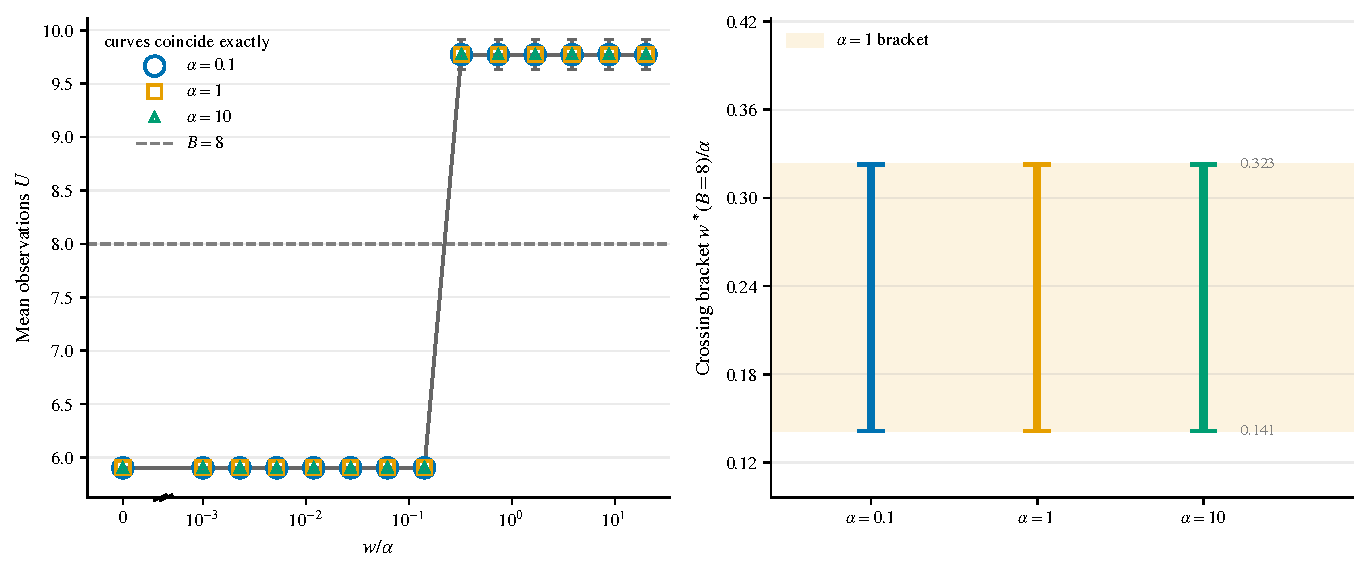
\includegraphics[width=\textwidth]{price_scale_invariance.pdf}
\caption{Curve collapse on Diagnosis. Left: $U$ vs.\ $w/\alpha$ at three reward scales. Right: crossing brackets of $B{=}8$ in $w/\alpha$ units coincide across scales (set-valued shadow price).}
\label{fig:collapse}
\end{figure}

\subsection{Proposition~2 onset on positive-threshold testbeds}
\label{sec:prop2}

Standard Tiger / Testbed parameters yield \emph{negative} $w_{\mathrm{thresh}}$, so any $w\ge 0$ observes and the duality check is vacuous. We therefore construct positive-threshold InfoSeeking environments ($p\in\{0.60,0.58\}$, $c{=}0.3$, $R_\pm=\pm 1$) with closed forms $w_{\mathrm{thresh}}\approx 3.44$ and $7.55$. A refined weight grid around the threshold shows $U{=}0$ at and below $w_{\mathrm{thresh}}$, with onset in $(w_{\mathrm{thresh}},\,1.03\cdot w_{\mathrm{thresh}}]$ on both environments (upper relative error $3\%$; Figure~\ref{fig:prop2}). Negative-threshold sanity checks on standard Testbed and Tiger remain consistent ($U(0)>0$ when $w_{\mathrm{thresh}}<0$).

\begin{figure}[t]
\centering
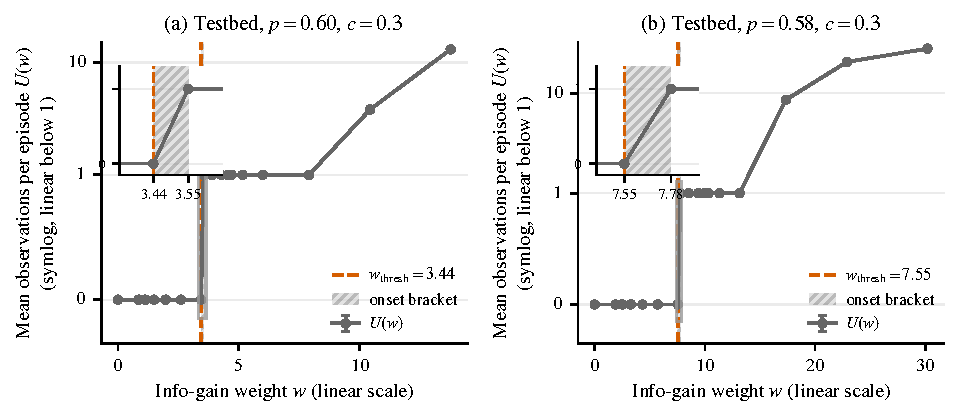
\includegraphics[width=\textwidth]{price_prop2_jumps.pdf}
\caption{Onset of observing on positive-threshold testbeds. Orange: H${=}1$ closed form~\eqref{eq:prop2}. Green band: empirical onset bracket after grid refinement.}
\label{fig:prop2}
\end{figure}

\subsection{Online dual control under reward rescale}
\label{sec:dual}

On Diagnosis with target $B{=}8$, learning rate $\eta_0{=}0.05$ and decay $\delta{=}0.02$, the dual controller pins rolling usage near the budget for $400$ episodes (Figure~\ref{fig:dual}). At episode~$200$ all rewards and costs are multiplied by~$10$ while $w$ is left unchanged. Usage drops, then recovers as $w$ climbs; windowed mean $w$ near the end of each half rises from $0.29$ to $2.71$ (ratio $9.3\approx 10$), matching~\eqref{eq:scale}.

The online and offline solutions agree in a stronger, set-valued sense as well. The shaded band in Figure~\ref{fig:dual} is the offline Diagnosis $\alpha{=}1$ crossing bracket $(0.141,0.323]$ for $B{=}8$, not a point estimate. The pre-rescale controller settles \emph{inside} that bracket ($0.29$), and the post-rescale controller settles at $2.71$---inside the $\times 10$-scaled bracket $(1.41,3.23]$ predicted by~\eqref{eq:scale}. The controller thus lands in the offline solution set at both reward scales without access to the usage curve, and the $9.3$ ratio is a consequence rather than a coincidence.

Learning-rate decay stabilizes the steady state but slows re-adaptation after the rescale. Measuring re-adaptation as the episodes from rescale until rolling-20 usage stays within $\pm 1$ of~$B$ for $20$ consecutive episodes, decay-only recovers in $157$ episodes. Enabling the shift detector (window~$20$, $k{=}3$, absolute floor $0.5$) fires a single lr reset at episode~$217$ and cuts re-adaptation to $45$ episodes (Figure~\ref{fig:dualreset}). Detection thresholds are a design choice; the point is that the stated remedy works under a simple, transparent rule.

\begin{figure}[t]
\centering
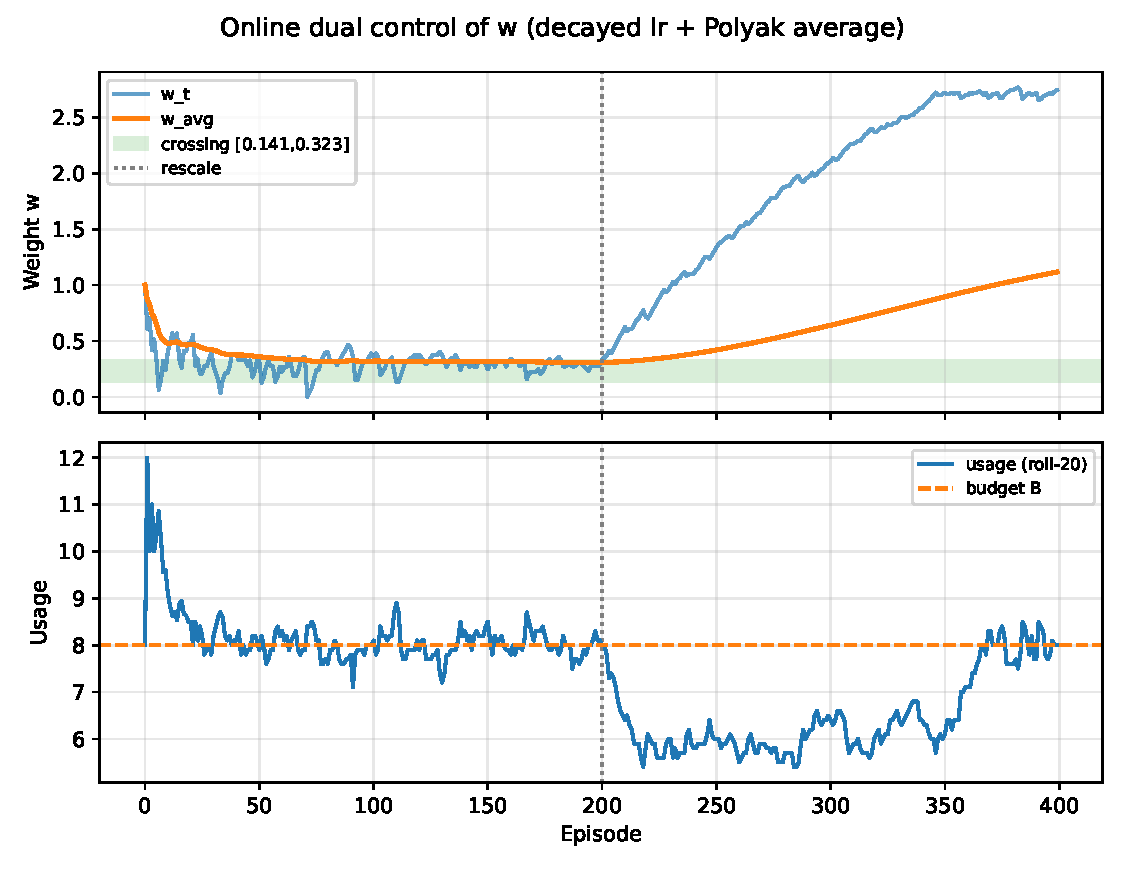
\includegraphics[width=0.85\textwidth]{price_dual_descent.pdf}
\caption{Dual control of $w$ on Diagnosis. Top: $w_t$, Polyak $w_{\mathrm{avg}}$, and offline crossing bracket. Bottom: rolling usage vs.\ budget. Vertical line: $\times 10$ reward rescale.}
\label{fig:dual}
\end{figure}

\begin{figure}[t]
\centering
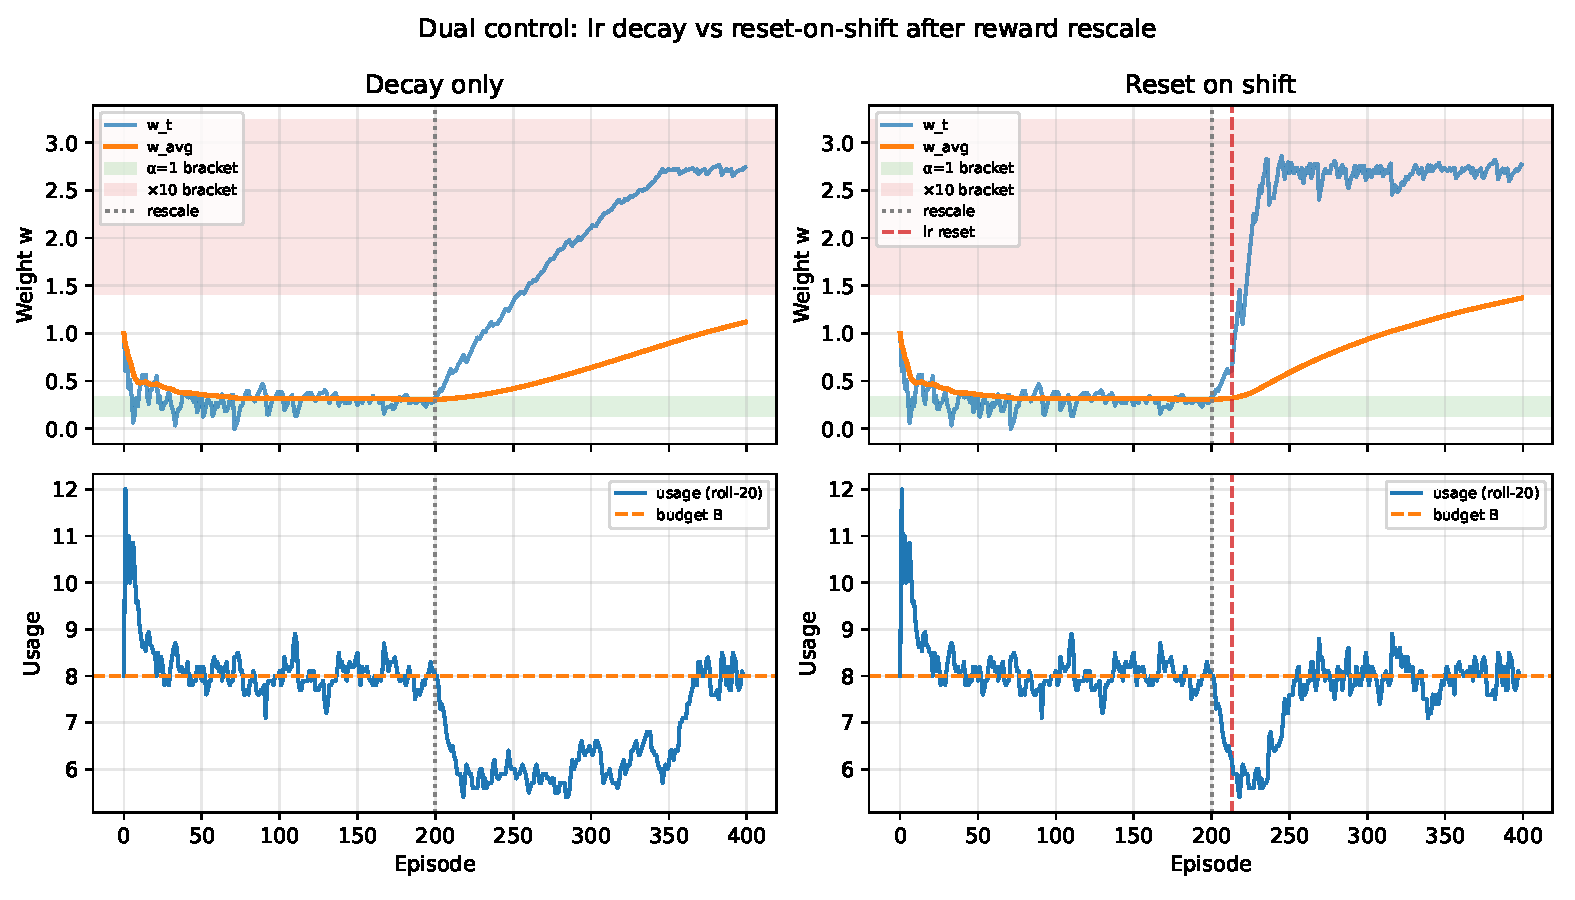
\includegraphics[width=\textwidth]{price_dual_reset.pdf}
\caption{Decay-only (left) vs.\ reset-on-shift (right) after the mid-run $\times 10$ rescale. Red dashed line: lr reset. Both controllers land in the $\times 10$ offline bracket; reset recovers the budget in $45$ episodes vs.\ $157$ under decay alone.}
\label{fig:dualreset}
\end{figure}

\subsection{Supporting: shadow-price staircases}
\label{sec:stairs}

Figure~\ref{fig:stairs} reports $w^*(B)$ over identifiable budgets inside $[U_{\min},U_{\max}]$ for Tiger, Diagnosis, Bandit, Tileworld-$6{\times}6$, and Inspection-$N{=}8$. Bandit and Inspection are roughly monotone with sensible brackets; Tiger, Diagnosis, and Tileworld show local non-monotonicity from discrete policy switches, so we report brackets and standard errors rather than singleton prices. Tiger's price is weakly identified: instrumental listening already saturates most of the usage range at $w{=}0$.

\begin{figure}[t]
\centering
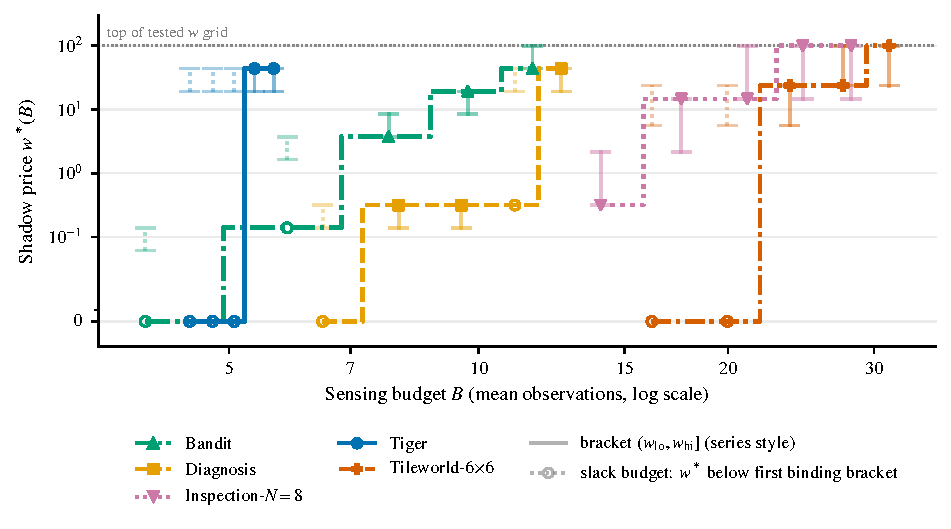
\includegraphics[width=0.85\textwidth]{price_shadow_curves.pdf}
\caption{Operational shadow-price staircases with vertical crossing brackets.}
\label{fig:stairs}
\end{figure}

Implicit EFE budgets $B_{\mathrm{EFE}}=U(w{=}1)$ on the same suite are: Tiger $4.21\pm 0.07$, Diagnosis $9.68\pm 0.15$, Bandit $5.03\pm 0.17$, Tileworld-$6{\times}6$ $14.83\pm 0.22$, Inspection-$N{=}8$ $18.24\pm 0.19$.

%----------------------------------------------------------------------
\section{Discussion and limitations}
\label{sec:discussion}
%----------------------------------------------------------------------

The three headline results jointly support reading $w$ as a budget-derived, scale-correct price of information. Curve collapse and coinciding brackets make the scale story visual; Proposition~2 onset ties the dual formulation back to the closed-form theory of the companion paper; and the dual controller independently converges into the offline crossing bracket at both reward scales, showing the online and offline views of the shadow price agree as sets, not just as ratios.

Limitations. (i)~At gap budgets the shadow price is set-valued---report brackets, not argmins. (ii)~$U(w)$ is only roughly monotone; grid solve with SEs is the default. (iii)~Budgets below $U(0)$ are unachievable with nonnegative~$w$ (instrumental sensing). (iv)~Shift detection thresholds ($k$, window, absolute floor) are design choices; we report one working setting rather than a full sensitivity sweep. (v)~We have not yet reported cost-usage curves alongside count usage.

Operationally, the designer's question becomes ``how much sensing can we afford?'' rather than ``what should $w$ be?'' EFE's $w{=}1$ is then the special case that buys $B_{\mathrm{EFE}}$ at the ambient scale---useful as a default, and now equipped with a budgeted escape hatch when the scale changes.

%----------------------------------------------------------------------
\section{Conclusion}
%----------------------------------------------------------------------

We recast the Planning+IG / EFE information weight as an operational shadow price of a sensing budget, with offline curve solves, set-valued crossing brackets, and an online dual controller. Empirically, usage curves collapse across reward scales, Proposition~2 onset matches the closed form to within~$3\%$, and dual control tracks a budget through a $\times 10$ reward rescale, landing inside the scaled offline bracket with $w$ ratio~$\approx 9.3$; lr reset-on-shift cuts re-adaptation from $157$ to $45$ episodes. The price of information, in this sense, is whatever $w$ the budget requires.

\subsubsection*{Acknowledgements}
This is a first draft extending~\citep{cooper2026efe}; venue and anonymization TBD.

%----------------------------------------------------------------------
\begin{thebibliography}{99}

\bibitem{altman1999}
E.~Altman.
\newblock {\em Constrained Markov Decision Processes}.
\newblock Chapman \& Hall/CRC, 1999.

\bibitem{araya2010}
M.~Araya, O.~Buffet, V.~Thomas, and F.~Charpillet.
\newblock A {POMDP} extension with belief-dependent rewards.
\newblock In {\em Advances in Neural Information Processing Systems}, 2010.

\bibitem{bernardo1979}
J.~M. Bernardo.
\newblock Expected information as expected utility.
\newblock {\em The Annals of Statistics}, 7(3):686--690, 1979.

\bibitem{cooper2026efe}
P.~Cooper.
\newblock Expected free energy as belief-dependent utility for $\rho$-{POMDPs}.
\newblock In {\em International Workshop on Active Inference (IWAI)}, 2026.
\newblock Accepted; companion paper.

\bibitem{fehr2018}
M.~Fehr, O.~Buffet, V.~Thomas, and J.~Dibangoye.
\newblock $\rho$-{POMDPs} have {Lipschitz}-continuous {Fr\'echet} derivatives.
\newblock In {\em Advances in Neural Information Processing Systems}, 2018.

\bibitem{friston2015}
K.~Friston, F.~Rigoli, D.~Ognibene, C.~Mathys, T.~Fitzgerald, and G.~Pezzulo.
\newblock Active inference and epistemic value.
\newblock {\em Cognitive Neuroscience}, 6(4):187--214, 2015.

\bibitem{haarnoja2018sac}
T.~Haarnoja, A.~Zhou, K.~Hartikainen, G.~Tucker, S.~Ha, J.~Tan, V.~Kumar, H.~Zhu, A.~Gupta, P.~Abbeel, and S.~Levine.
\newblock Soft actor-critic algorithms and applications.
\newblock arXiv:1812.05905, 2018.

\bibitem{matejka2015}
F.~Mat\v{e}jka and A.~McKay.
\newblock Rational inattention to discrete choices: A new foundation for the multinomial logit model.
\newblock {\em American Economic Review}, 105(1):272--298, 2015.
\newblock doi:10.1257/aer.20130047.

\bibitem{parr2019}
T.~Parr and K.~J. Friston.
\newblock Generalised free energy and active inference.
\newblock {\em Biological Cybernetics}, 113(5--6):495--513, 2019.

\bibitem{sims2003}
C.~A. Sims.
\newblock Implications of rational inattention.
\newblock {\em Journal of Monetary Economics}, 50(3):665--690, 2003.
\newblock doi:10.1016/S0304-3932(03)00029-1.

\end{thebibliography}

\end{document}
